 \documentclass[12pt,a4paper]{article}

\usepackage{graphicx}% Include figure files
\usepackage{dcolumn}% Align table columns on decimal point
\usepackage{bm}% bold math
%\usepackage{hyperref}% add hypertext capabilities
%\usepackage[mathlines]{lineno}% Enable numbering of text and display math
%\linenumbers\relax % Commence numbering lines

%\usepackage[showframe,%Uncomment any one of the following lines to test 
%%scale=0.7, marginratio={1:1, 2:3}, ignoreall,% default settings
%%text={7in,10in},centering,
%%margin=1.5in,
%%total={6.5in,8.75in}, top=1.2in, left=0.9in, includefoot,
%%height=10in,a5paper,hmargin={3cm,0.8in},
%]{geometry}

\usepackage{multicol}%Para hacer varias columnas
\usepackage{multicol,caption}
\usepackage{multirow}
\usepackage{cancel}
\usepackage{hyperref}
\hypersetup{
    colorlinks=true,
    linkcolor=blue,
    filecolor=magenta,      
    urlcolor=cyan,
}

\setlength{\topmargin}{-1.0in}
\setlength{\oddsidemargin}{-0.3pc}
\setlength{\evensidemargin}{-0.3pc}
\setlength{\textwidth}{6.75in}
\setlength{\textheight}{9.5in}
\setlength{\parskip}{0.5pc}

\usepackage[utf8]{inputenc}
\usepackage{expl3,xparse,xcoffins,titling,kantlipsum}
\usepackage{graphicx}
\usepackage{xcolor} 
\usepackage{siunitx}
\usepackage{nopageno}
\usepackage{lettrine}
\usepackage{caption}
\renewcommand{\figurename}{Figura}
\usepackage{float}
\renewcommand\refname{Bibliograf\'ia}
\usepackage{amssymb}
\usepackage{amsmath}
\usepackage[rightcaption]{sidecap}
\usepackage[spanish]{babel}

\providecommand{\abs}[1]{\lvert#1\rvert}
\providecommand{\norm}[1]{\lVert#1\rVert}
\newcommand{\dbar}{\mathchar'26\mkern-12mu d}

\usepackage{mathtools}
\DeclarePairedDelimiter\bra{\langle}{\rvert}
\DeclarePairedDelimiter\ket{\lvert}{\rangle}
\DeclarePairedDelimiterX\braket[2]{\langle}{\rangle}{#1 \delimsize\vert #2}

% CABECERA Y PIE DE PÁGINA %%%%%
\usepackage{fancyhdr}
\pagestyle{fancy}
\fancyhf{}

\begin{document}

Macías Márquez Misael Iván

\begin{enumerate}



%%%1%%%



\item En la figura 1, si el haz (1) es el haz incidente. ¿Cuáles de los otros cuatro rayos son haces reflejados? y ¿cuáles son haces refractados?


\begin{figure}[h!]
    \centering
    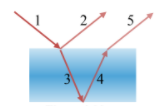
\includegraphics{1.PNG}
    \caption{}
    \label{fig:my_label}
\end{figure}

\textbf{Res:} Los rayos reflejados son 2 y 4 ya que tienen el mismo ángulo con la normal que el rayo incidente que les corresponde, que serían el 1 y 3 respectivamente, los ángulos refractados son 3 y 5 debido a que sus ángulos formados con respecto a la normal no son iguales a sus rayos de incidencia (1 y 4 respectivamente), también se puede ver que el rayo viaja a una menor velocidad en el medio azul ya que en ángulo con la normal de 3 es menor al 1 y porque el ángulo con la normal de 5 es mayor al 4.





%%%2%%%






\item Supongamos que se tiene una superficie reflectora elíptica como la mostrada en la figura 2. ¿Cuál es la trayectoria con tiempo mínimo (o estacionario) para ir de un foco ($A$) de la elipse al otro foco ($B$) a través de una reflexión en la superficie?

\begin{figure}[h!]
    \centering
    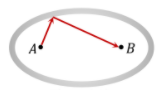
\includegraphics{2.PNG}
    \caption{}
    \label{fig:my_label}
\end{figure}

\textbf{Sol:} 

Sea $X$ un punto en la superficie reflectora, entonces para encontrar la trayectoria se usa el principio de Fermat para minimizar la trayectoria entre $AXB$ ya que no hay cambio de medio y por tanto cambio de velocidad,

\begin{equation*}
    d(AXB) = d(A,X) + d(X,B)
\end{equation*}

pero como $A$ y $B$ son los focos de la superficie y al tenerse una elipse, se cumple que

\begin{equation*}
    d(AXB) = 2a = cte
\end{equation*}

donde $a$ es la medida del semieje mayor, y entonces

\begin{equation*}
    \frac{\partial d(AXB)}{\partial x} = 0
\end{equation*}

por lo tanto no existe una única trayectoria con tiempo mínimo para ir de $A$ a $B$ pasando por una reflexión en la superficie elíptica.




%%%3%%%




\item Supongamos que se tiene un material translucido circular (figura 3). ¿En qué posición, dentro del material, habría que colocar una fuente puntual para que los rayos de la luz salieran del mismo como si el material no estuviera presente? (Es decir, que los frentes de onda preservarán su geometría circular).

\begin{figure}[h!]
    \centering
    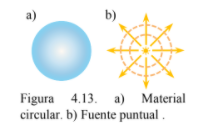
\includegraphics{3.PNG}
    \caption{}
    \label{fig:my_label}
\end{figure}

\textbf{Res:} Suponiendo que el material por sus dos caras es liso, la fuente debe estar en el centro del material ya que al ser una fuente puntual con frente de "onda" esférico y al tenerse un material con superficie esférica, el ángulo entre la normal y el rayo incidente sería nulo para cualquier rayo y por la ley de Snell el ángulo de refracción también sería nulo, lo mismo pasa con la superficie exterior del material. Si el grosor en la el cascarón del material no es homogéneo y por tanto se tiene una superficie irregular, la posición de la fuente ya no sería necesariamente el centro y esta dependería completamente de la distribución del material en el cascarón.


 



%%%4%%%




\item En un experimento se observa que cuando un haz pasa de agua a diamante (incidiendo a un ángulo de $45^{\circ}$) se refracta a un ángulo de $23.1^{\circ}$. ¿En qué material viaja más rápido la luz?.

\textbf{Sol:}

Sabemos por la ley de Snell que

\begin{equation*}
    n_T \sin{\theta_T} = n_I \sin{\theta_I}
\end{equation*}

donde $\theta_I$ es el ángulo de incidencia y $\theta_T$ es el ángulo de refracción, también $n_T= c/v_T$ y $n_I = c/v_I$, entonces

\begin{equation}
    \frac{c}{v_T} \sin{\theta_T} = \frac{c}{v_I} \sin{\theta_I} \hspace{0.3cm} \rightarrow  \hspace{0.3cm} \frac{v_I}{v_T}  = \frac{\sin{\theta_I}}{\sin{\theta_T}} 
\end{equation}

que sustituyendo

\begin{equation*}
    \frac{v_I}{v_T}  = \frac{\sin{45^{\circ}}}{\sin{23.1^{\circ}}} \approx  1.81
\end{equation*}

por lo tanto $\frac{v_I}{v_T} >1$ o bien $v_I > v_T$, entonces la luz viaja más rápido en el agua.



%%%5%%%




\item En otro experimento, un rayo que pasa de vidrio tipo Flint a lucita (incidiendo a $45^{\circ}$) se refracta a un ángulo de $49.4^{\circ}$. ¿En qué material la luz es más rápida?.

\textbf{Sol:}

Usando de nuevo la ecuación 1 tenemos que

\begin{equation*}
    \frac{v_I}{v_T}  = \frac{\sin{\theta_I}}{\sin{\theta_T}}  =\frac{\sin{45^{\circ}}}{\sin{49.4^{\circ}}} \approx 0.93
\end{equation*}

por lo tanto $\frac{v_I}{v_T} <1$ o bien $v_I < v_T$, entonces la luz viaja más rápido en la lucita.






%%%6%%%




\item Asumiendo que se conoce la velocidad de la luz en uno de los medios, ¿Cómo se puede linealizar la ecuación (4.7)?, ¿cómo se puede conocer la velocidad de la luz del otro medio a partir de la linealización?.

\textbf{Res:} Supongamos que se conoce la velocidad del medio incidente ($v_I$), se puede linealizar de muchas formas la ecuación 4.7 que resulta ser la ecuación 1 del ejercicio 4, por ejemplo sea $x = \sin{\theta_I}$, $m=v_T$ , $y= v_I \sin{\theta_T}$ y $b=0$, entonces la ecuación 1 toma la forma de una ecuación general de recta para una variable $y=mx +b$.



Para determinar la velocidad del otro medio $v_T$ se puede usar el método de mínimos cuadrados para ajustar la pendiente de la ecuación linealizada midiendo los ángulos de incidencia y refracción.








%%%7%%%




\item Asumiendo que el ángulo $\theta$ se puede medir directamente con incertidumbre $\Delta \theta$. ¿Cuál será la incertidumbre de la función $\sin{(\theta)}$?

\textbf{Sol:}

Sea $f= \sin{\theta}$, por la regla de derivación y suma por cuadraturas en la propagación de incertidumbres,

\begin{equation*}
    \Delta \theta = \sqrt{\left(\frac{\partial f}{\partial \theta}\right)^2 \Delta \theta^2} = |\cos{\theta}| \Delta \theta
\end{equation*}

    
    
\end{enumerate}

\end{document}